
\documentclass[10pt]{beamer}
\mode<presentation>
{
  \usetheme{Warsaw}    
  \usecolortheme{seahorse} 
 \usefonttheme{serif}
 \setbeamersize{text margin left=10mm,text margin right=10mm}
 \setbeamertemplate{headline}{}
}


% Display formulas and symbols
%%---------------------------------
\usepackage{amsmath}

% Graphics, subfigures, captions (+ subcaptions)
%%---------------------------------
\usepackage{graphicx}
\usepackage{subcaption}
\usepackage{caption}

% Tables
%%---------------------------------
\usepackage{tabularx}
\usepackage{booktabs}

% Bibliography
%%---------------------------------
\usepackage[backend=bibtex,
            sortcites=true,
            sorting=nyt,
            citetracker=false,
            %ibidtracker=false,
            style=authoryear,
            %doi=true,
            %isbn=false,
            giveninits=true,
            uniquename=init,
            maxnames=3]{biblatex}
            
% Reduce fontsize of references
\renewcommand*{\bibfont}

% Load bibliography
\addbibresource{references.bib}

%%---------------------------------
\title{Explore the multifaceted determinants of regional employment rates in Germany}
\subtitle{\textit{How do economic performance, labor market dynamics, educational attainment, and industry composition affect regional employment rates in Germany?}} % \textbf{} for bold text...
\author{Stephen Elvis Ampah \href{mailto:elvis.ampah@tu-dortmund.de}{elvis.ampah@tu-dortmund.de}}
\institute{Technische Universität Dortmund - Ruhr Alliance, Germany}
\date{\today}

\setbeamertemplate{navigation symbols}{}
\setbeamertemplate{footline}{
    \leavevmode%
    \hbox{%
    \begin{beamercolorbox}[wd=.5\paperwidth,ht=2.25ex,dp=1ex,left]{author in head/foot}%
        \usebeamerfont{author in head/foot}\hspace*{2ex}Stephen Elvis Ampah \hfill \texttt{\href{mailto:elvis.ampah@tu-dortmund.de}{elvis.ampah@tu-dortmund.de}}\hspace*{2ex}
    \end{beamercolorbox}%
    \begin{beamercolorbox}[wd=.5\paperwidth,ht=2.25ex,dp=1ex,right]{title in head/foot}%
        \usebeamerfont{title in head/foot}\insertframenumber{} / \inserttotalframenumber\hspace*{2ex}
    \end{beamercolorbox}}%
    \vskip0pt%
}

% Here starts the actual presentation + slides
%%---------------------------------
%%---------------------------------

\usepackage{Sweave}
\begin{document}
\Sconcordance{concordance:S_E_Ampah_QRE.tex:S_E_Ampah_QRE.Rnw:1 71 1 1 0 2 1 1 21 1 1 %
1 6 3 1 1 12 1 1 1 8 1 1 1 6 3 1 1 12 1 1 1 15 1 1 1 9 10 1 1 22 10 1 1 %
6 1 1 1 6 7 1 1 41 5 1 1 21 4 1 1 17 5 1 1 5 1 1 1 15 1 1 1 6 5 1 1 29 %
1 9 5 1 1 31 1 1 1 5 4 1 1 18 1 1 1 23 1 1 1 14 8 1 1 12 1 1 1 31 8 1 1 %
18 1 1 1 8 1 1 1 13 6 1 1 7 1 1 1 5 1 1 1 8 1 1 1 9 1 1 1 14 6 1 1 29 %
164 1 1 10 1 2 7 1 1 3 1 2 7 1 1 19 1 2 8 1 1 9 1 2 7 1 1 13 1 2 195 1 %
1 28 1 2 51 1}





% \section{Data Manipulation}
% Data manipulation is crucial for preparing the dataset for analysis. This includes renaming columns for better clarity and handling data types appropriately.






% \section{Handling Missing Data}
% This section deals with identifying and imputing missing data points in the dataset to prepare it for further analysis.







% \section{Density and Correlation Analysis}
% 
% This section focuses on understanding the distribution of various numeric variables and their interrelationships within the dataset.
% 
% <<density-plot-single, echo=TRUE, echo=F, fig=TRUE, fig.cap="Density plot of ER_2021", fig.align='center'>>=
% plot(density(final_inkar_data$ER_2021), main="Density of ER_2021", xlab="ER_2021 Values", ylab="Density")
% @
% 
% 


% <<apply-density-function, echo=FALSE, fig=TRUE, fig.cap="Density plots for numeric variables", fig.align='center'>>=
% plot_all_densities(final_inkar_data)
% @


% \section{Data Transformation and Re-Imputation}
% 
% This section discusses the log transformation of specific variables in the dataset, followed by a re-imputation process to handle any newly introduced missing values resulting from the transformation.




% 
% \section{Regression Analysis}
% 
% This section presents the Ordinary Least Squares (OLS) regression analysis conducted for each year from 2009 to 2021. The models predict the Employment Rate ('ER') using various predictors across different years.
% Each model predicts 'ER' (Employment Rate) using variables 'HEEQ' (Higher Education Enrollment Quota), 'EKII' (Employees in Knowledge-Intensive Industries), 'HI' (Household Income),
% 'UR' (Unemployment Rate), and 'GDP' (Gross Domestic Product).



% \section{Variance Inflation Factor (VIF) Analysis}
% 
% To ensure the reliability of our models, the Variance Inflation Factor (VIF) was calculated for each, helping to identify any significant multicollinearity issues that could impact our interpretations.


% \section{Spatial Data Integration and Visualization}
% 
% This section focuses on integrating spatial data with our main dataset and visualizing the results to provide geographic insights into the Employment Rate (ER) data for the year 2021.
% 


% \section{Data Transformation for Spatiotemporal Modeling}
% 
% This section details the transformation of our dataset into a format suitable for spatiotemporal modeling, focusing on converting the dataset from wide to long format and manipulating variable names to extract time-related information.
% 






% \section{Summary Statistics Calculation}
% 
% This section details the computation of various summary statistics for selected columns of our dataset. These statistics include mean, median, standard deviation, standard error, minimum, maximum, and quantiles.
% 



% \section{Spatial Model Preparations}
% 
% This section focuses on preparing the spatial data for subsequent analysis, including creating neighbors lists and constructing spatial weights matrices, which are crucial for spatial econometrics.
% 


 
% \section{Testing for Spatial Autocorrelation}
% 
% This section details the process of checking for spatial autocorrelation using Moran's I test across multiple years. This test helps determine if a spatial econometric model is necessary by identifying patterns of autocorrelation in the residuals of ordinary least squares (OLS) models.
% 




% \section{Conclusion}
% 
% The Moran's I test results across multiple years indicate the presence of spatial autocorrelation in the residuals of the OLS models. These findings inform the necessity and design of spatial econometric models to account for spatial dependencies. 
% 
% 
% \section{Creating Spatially Lagged Variables}
% 
% This section details the creation and processing of spatially lagged variables to account for spatial autocorrelation in the dataset. These variables help in capturing the influence of neighboring observations on each other, which is crucial for spatial analyses.




% \section{Conclusion}
% 
% Incorporating spatially lagged variables enhances our model's ability to account for spatial dependencies, thereby improving the robustness and accuracy of our spatial analyses. This step is essential in ensuring that our model reflects the real-world spatial processes influencing our variables of interest.
% 
% \section{Reformatting Data for Spatiotemporal Analysis}
% 
% This section details the reformatting of our dataset to include newly created spatially lagged variables, preparing it for advanced spatiotemporal modeling.






% \section{Conclusion}
% The dataset has been successfully transformed to include spatially lagged variables and formatted for spatiotemporal modeling using the splm package. These steps are critical for ensuring the accuracy and robustness of our forthcoming analyses.

% \section{Spatial Econometric Modeling}
% This section focuses on fitting spatial econometric models to our data to account for possible spatial autocorrelation. We explore both the Spatial Lag Model (SLM) and the Spatial Error Model (SEM) to evaluate their impacts on the analysis.










% \section{Conclusion}
% Spatial econometric models, specifically the SLM and SEM, provide insights into the spatial dependencies within our data. Calculating the impacts of these models helps in understanding the influence of spatial spillovers on the estimated parameters, ensuring a deeper understanding of the underlying spatial processes

% \section{Diagnostic Plots for Spatial Models}
% This section includes diagnostic plots for the Spatial Lag Model (SLM) and Spatial Error Model (SEM). These plots provide insights into the residuals and fit of the models, which are crucial for evaluating model performance and identifying potential issues.


% \section{Conclusion}
% 
% The diagnostic plots provide essential visual feedback on the residuals and fit of our spatial econometric models. These visual diagnostics are key to assessing model adequacy, guiding further refinements and validations of the model specifications.


% Slide 1
\begin{frame}[plain]
\titlepage
\end{frame}

% Table of Contents
\begin{frame}{Table of Contents}
\tableofcontents
\end{frame}


% Slide 2 - Importance of Studying Regional Employment Rates
\section{Introduction}
\begin{frame}{Introduction}
    \setlength{\parskip}{1em}  
    \textbf{Importance of Studying Regional Employment Rates}
    \begin{itemize}
        \item \textbf{Economic Health Indicator:} Employment rates are critical indicators of economic health and labour market performance
        \item \textbf{Policy Relevance:} Understanding regional variations in employment can guide targeted policy interventions 
        \item \textbf{Social Implications:} High employment rates are associated with better social outcomes, including reduced poverty and improved quality of life \parencite{moller2010}.
    \end{itemize}
\end{frame}


% Slide 3 - Research Question
\begin{frame}{Research Question}
    \setlength{\parskip}{1em}
    \textbf{Research Question}
    \begin{itemize}
        \item \textbf{} How do economic performance, labour market dynamics, educational attainment, and industry composition affect regional employment rates in Germany?
    \end{itemize}

    \textbf{Literature}
    \begin{itemize}
         \item How elastic is labor demand? A meta-analysis for the German labor market. \textit{Journal for Labour Market Research}, 57(1), 14. \parencite{Popp2023}.
         \item Another economic miracle? The German labor market and the Great Recession. \textit{IZA Journal of Labor Policy}, 1, 1-21. \parencite{RinneZimmermann2012}.
    \end{itemize}
\end{frame}


% Slide 4 - Methodology
\section{Methodology}
\begin{frame}{Methodology}
\frametitle{Data Sources}
    \setlength{\parskip}{1em}
    \begin{itemize}
        \item \textbf{INKAR.de}: A comprehensive database provided by the Federal Institute for Research on Building, Urban Affairs, and Spatial Development (BBSR) in Germany. 
        \item \textbf{Variables}:
        \begin{itemize}
            \item \textbf{Employment Rate (ER)}: Proportion of the working-age population that is employed.
            \item \textbf{Higher Education Enrollment Quota (HEEQ)}: Percentage of the population enrolled in higher education.
            \item \textbf{Employees in Knowledge-Intensive Industries (EKII)}: Share of employment in sectors requiring advanced knowledge and skills.
            \item \textbf{Household Income (HI)}: Average income of households.
            \item \textbf{Unemployment Rate (UR)}: Percentage of the labour force that is unemployed and seeking work.
            \item \textbf{Gross Domestic Product (GDP)}: Total economic output of a region.
        \end{itemize}
    \end{itemize}
\end{frame}


% Slide 5 - Baseline Model
\begin{frame}{Analytical Approach}
\frametitle{Baseline Model: Ordinary Least Squares (OLS) Regression}
    \begin{itemize}
        \item \textbf{Purpose}: Establish initial relationships between the dependent variable \( ER \) and independent variables \( HEEQ, EKII, HI, UR, GDP \).
        \item \textbf{Procedure}: Fit an OLS regression model to the data to determine the direct effects of the independent variables on the employment rate.
        \item \textbf{Formula}:
        \begin{equation}
            ER = \beta_0 + \beta_1 HEEQ + \beta_2 EKII + \beta_3 HI + \beta_4 UR + \beta_5 GDP + \epsilon
        \end{equation}
        where \( \beta_i \) are parameters to be estimated and \( \epsilon \) is the error term.
    \end{itemize}
    \textit{Note: The model formulation follows the guidelines set out in Wooldridge (2012).}
\end{frame}


% Slide 6
\begin{frame}{Moran's I Test \parencite{moran1950}}
    \begin{itemize}
        \item \textbf{Purpose}: Detect spatial patterns and autocorrelation in the residuals of the OLS model.
        \item \textbf{Formula}:
        \begin{equation}
            I = \frac{N}{W} \frac{\sum_{i} \sum_{j} w_{ij} (x_i - \bar{x})(x_j - \bar{x})}{\sum_{i} (x_i - \bar{x})^2}
        \end{equation}
        where:
        \begin{itemize}
            \item \(N\): Number of observations
            \item \(W\): Sum of all spatial weights \(w_{ij}\)
            \item \(x_i\): Value of the variable at location \(i\)
            \item \(x_j\): Value of the variable at location \(j\)
            \item \(\bar{x}\): Mean of the variable
            \item \(w_{ij}\): Spatial weight between location \(i\) and \(j\)
        \end{itemize}
        \item \textbf{Result}: Indicated patterns of spatial autocorrelation, suggesting that the employment rates in one district are influenced by those in neighbouring regions.
    \end{itemize}
\end{frame}

% Slide 7
\begin{frame}{Spatial Econometric Models}
    \begin{itemize}
        \item \textbf{Spatial Lag Model (SLM) \parencite{anselin1988}}:
        \begin{itemize}
            \item \textbf{Purpose}: Account for the dependence of employment rates in neighbouring district.
            \item \textbf{Method}: Incorporates a spatially lagged dependent variable to capture the influence of neighbouring district' employment rates on the local employment rate.
            \item \textbf{Equation}:
            \begin{equation}
                ER = \rho W ER + X \beta + \epsilon
            \end{equation}
            where:
            \begin{itemize}
                \item \(ER\): Employment rate in region 
                \item \(W\): The spatial weights matrix
                \item \(W ER\): Spatially lagged employment rate
                \item \(X\): Matrix of independent variables
                \item \(\beta\): The vector of coefficients for the independent variables
                \item \(\epsilon\): The vector of error terms
                \item \(\rho\): Spatial autoregressive coefficient
            \end{itemize}
        \end{itemize}
    \end{itemize}
\end{frame}


% Slide 8
\begin{frame}{Spatial Econometric Models (Robustness Test)}
    \begin{itemize}
     \item \textbf{Spatial Error Model (SEM)}:
    \begin{itemize}
        \item \textbf{Purpose}: Account for spatially correlated error terms.
        \item \textbf{Method}: Adjusts for spatial dependence in the error term, capturing unobserved district factors affecting employment rates.
        \item \textbf{Equation}:
        \begin{subequations}
          \begin{equation}
              ER = X\beta + u
          \end{equation}
          \begin{equation}
              u = \lambda Wu + \epsilon
          \end{equation}
          \end{subequations}
        where:
\begin{itemize}
  \item \( ER \) is the dependent variable vector
  \item \( X \) is the matrix of independent variables
  \item \( \beta \) is the vector of coefficients for the independent variables
  \item \( u \) is the vector of error terms that incorporates spatial autocorrelation
  \item \( \lambda \) is the coefficient of spatial autocorrelation for the error terms
  \item \( W \) is the spatial weights matrix
  \item \( \epsilon \) is the vector of independently and identically distributed (iid) error terms
\end{itemize}
    \end{itemize}
    \item \textit{The robustness of the SEM in comparison to SLM is discussed extensively in Spatial Econometrics \parencites{anselin1988}{elhorst2014}.}
\end{itemize}
\end{frame}


\section{Descriptive Analysis and Results}
\begin{frame}{Percentage of missing vs non-missing data points}
\begin{figure}
\begin{subfigure}[b]{0.6\textheight}
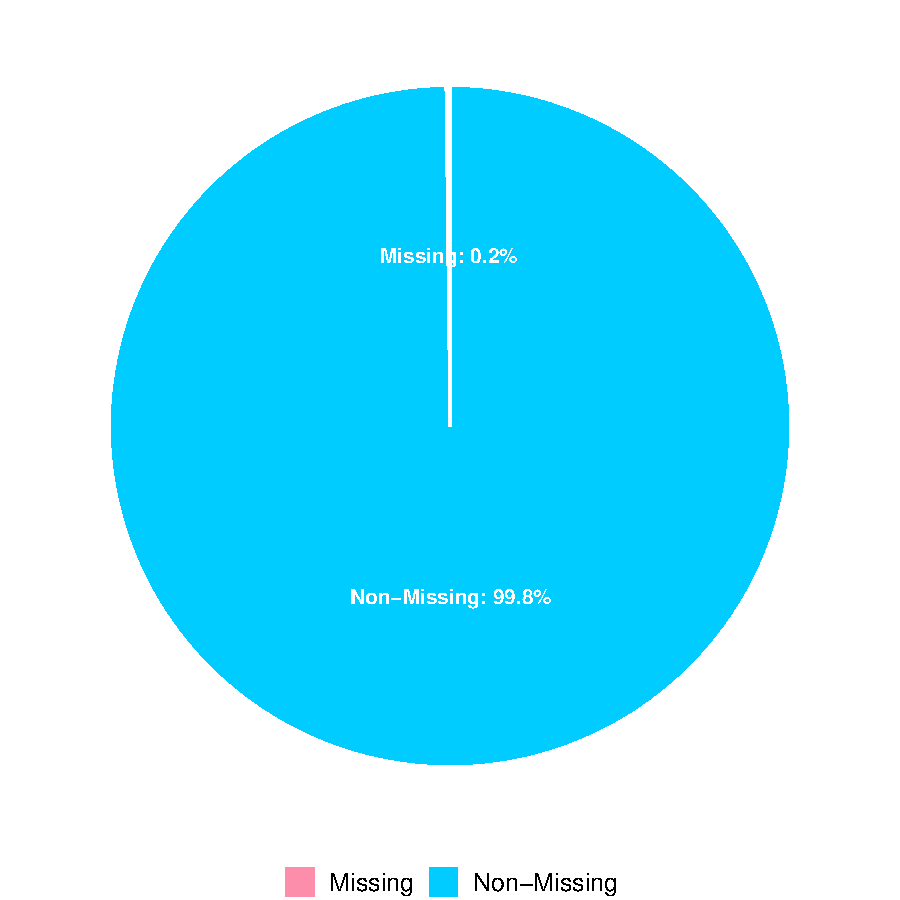
\includegraphics{S_E_Ampah_QRE-missing-data-visualization}
\end{subfigure}
% \caption{Percentage of missing vs non-missing data points}
\end{figure}
\end{frame}


\begin{frame}{Density Plots}
\begin{figure}
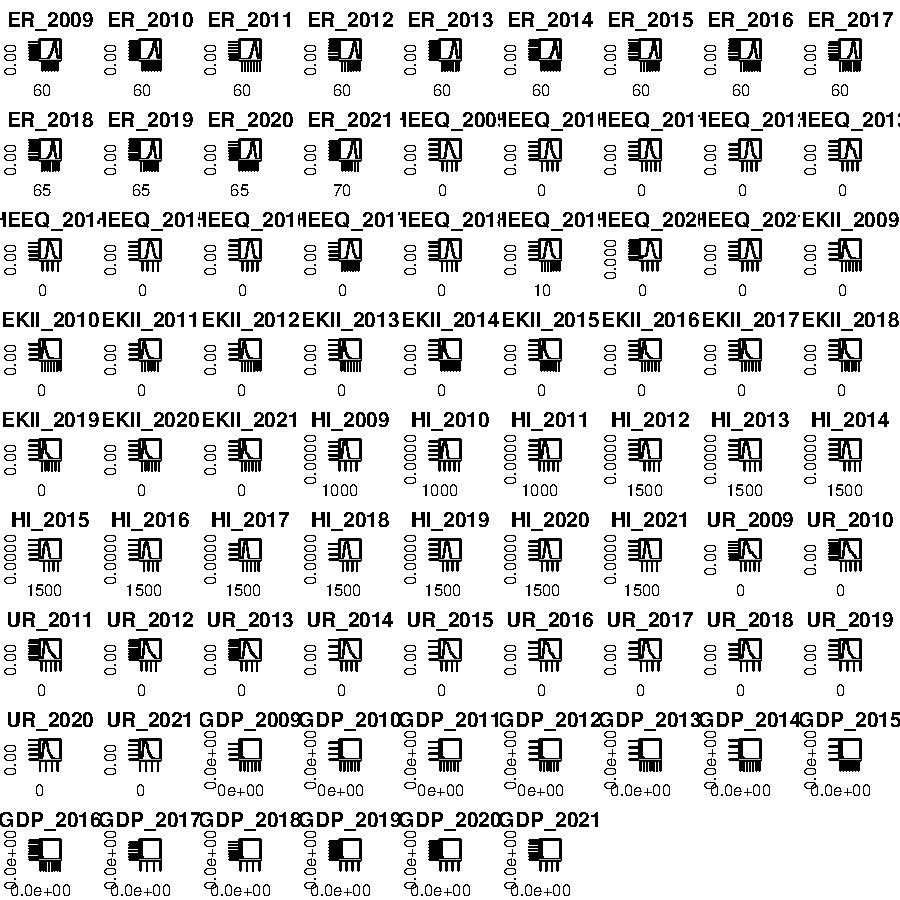
\includegraphics{S_E_Ampah_QRE-apply-density-function}
\caption{Density plots for numeric variables}
\end{figure}
\end{frame}


\begin{frame}[fragile]{Employmemt rate in Germany - 2021}
\begin{figure}
\begin{subfigure}[b]{1\textheight}
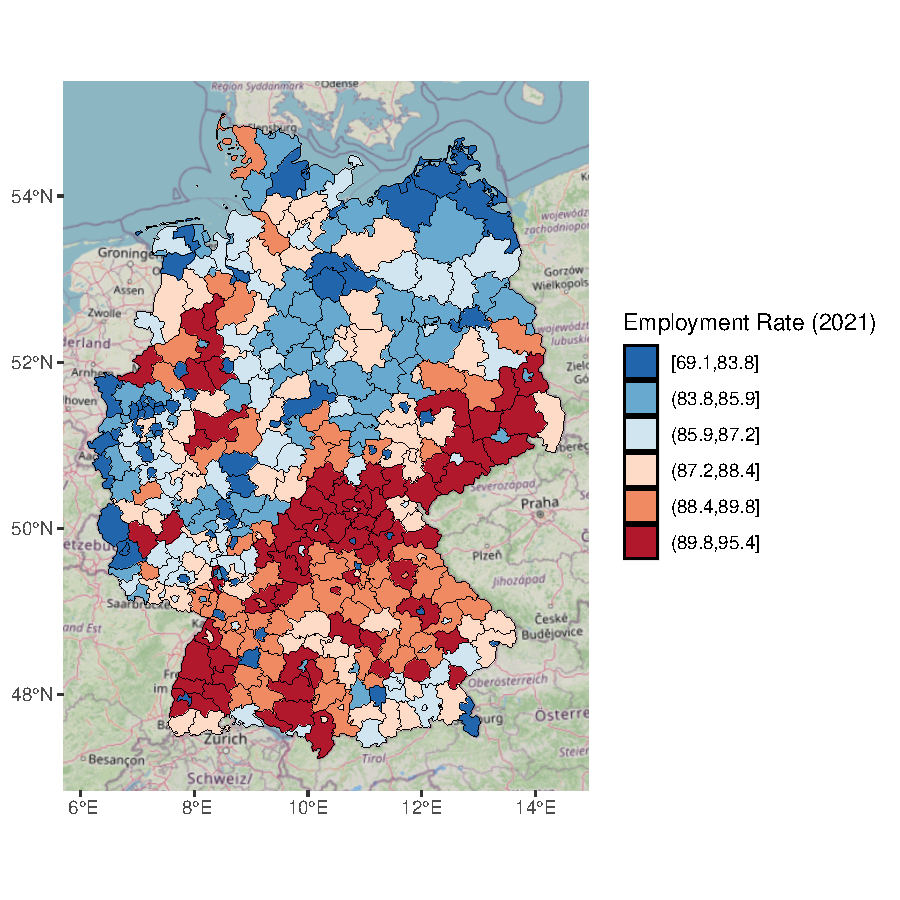
\includegraphics{S_E_Ampah_QRE-quantile-map-visualization}
\end{subfigure}
% \caption{Employmemt rate in Germany - 2021}
\end{figure}
\end{frame}


\begin{frame}{Neighborhood Structure (Spatial dependence)}
\begin{figure}
\begin{subfigure}[b]{1\textheight}
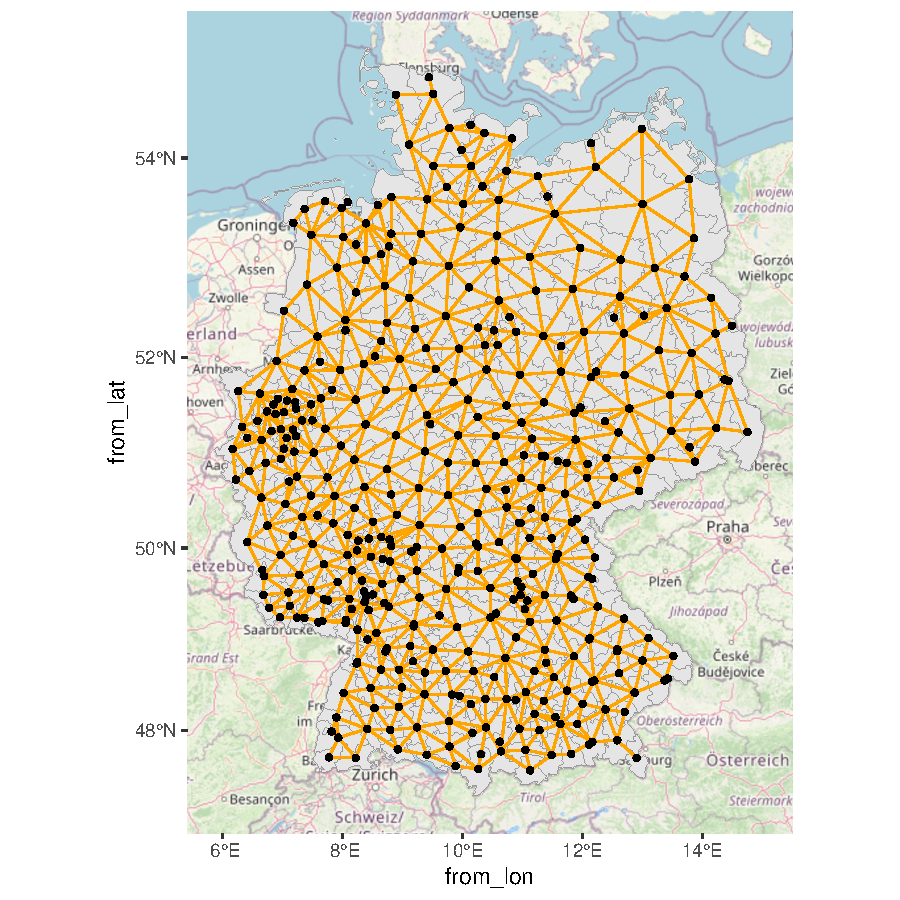
\includegraphics{S_E_Ampah_QRE-plot-spatial-data-neighbors}
\end{subfigure}
\end{figure}
\end{frame}


\begin{frame}[fragile]{Correlation Matrix of Numeric Variables}
\begin{figure}
\begin{subfigure}[b]{1\textheight}
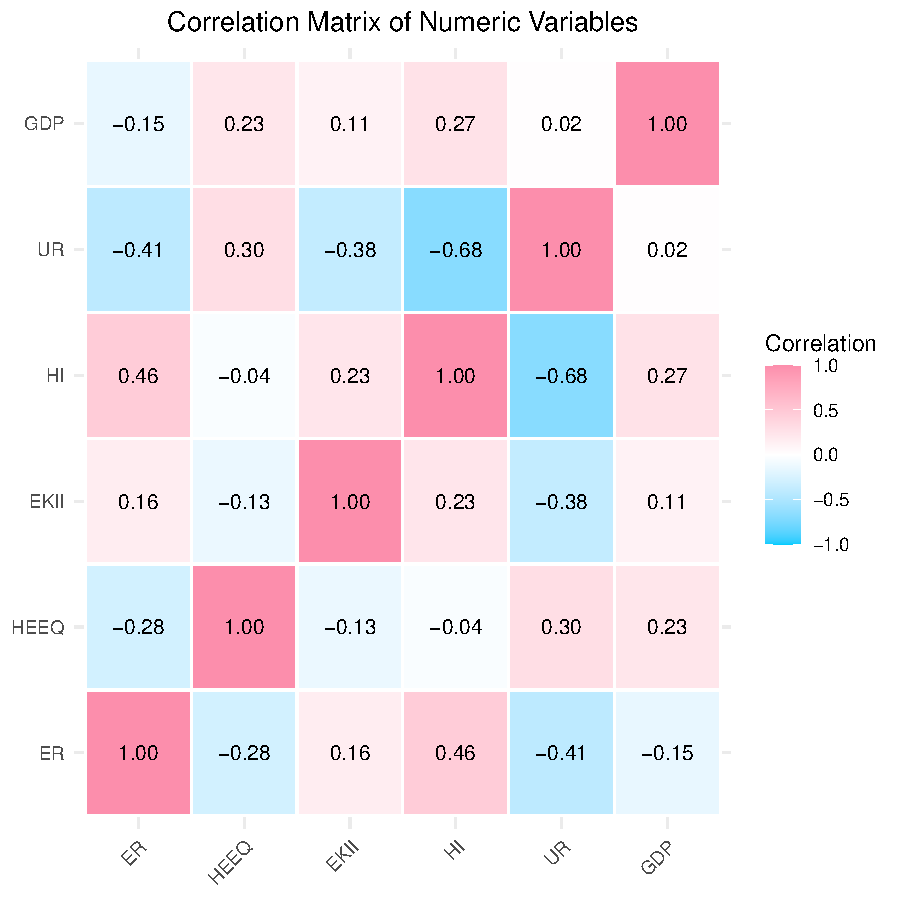
\includegraphics{S_E_Ampah_QRE-plot-Correlation-Matrix}
\end{subfigure}
% \caption{Correlation Matrix of Numeric Variables}
\end{figure}
\end{frame}


\begin{frame}{Descriptive Statistics for Various Variables}
\begin{table}[ht]
\centering
\small 
\begin{tabular}{@{}lccccccccc@{}}
\toprule
Variable & Mean & Median & SD & Min & Max & Q25 & Q75 & Skewness \\ 
\midrule
ER   & 4.41 & 4.42 & 0.05 & 4.09 & 4.57 & 4.38 & 4.45 & -0.77 \\
HEEQ & 3.41 & 3.44 & 0.38 & -2.81 & 4.25 & 3.23 & 3.64 & -4.35 \\
EKII & 2.12 & 2.15 & 0.74 & -1.47 & 4.04 & 1.71 & 2.61 & -0.63 \\
HI   & 7.47 & 7.47 & 0.14 & 7.09 & 8.14 & 7.37 & 7.56 & 0.12 \\
UR   & 1.68 & 1.69 & 0.47 & 0.22 & 2.88 & 1.33 & 2.02 & 0.00 \\
GDP  & 15.45 & 15.37 & 0.77 & 13.73 & 18.92 & 14.90 & 15.88 & 0.90 \\
\bottomrule
\end{tabular}
\end{table}
\end{frame}


\begin{frame}{OLS Regression Results}
\begin{table}[ht]
\centering
\begin{tabular}{@{}lcccc@{}}
\toprule
Variable & Estimate & Std. Error & t value & Pr(>|t|) \\ 
\midrule
(Intercept) & 3.32 & 0.04 & 75.07 & $<2.00e^{-16}$ *** \\
HEEQ        & -0.03 & 0.002 & -16.72 & $<2.00e^{-16}$ *** \\
EKII        & 0.00 & 0.001 & 4.43 & $9.51e^{-6}$ *** \\
HI          & 0.19 & 0.006 & 31.28 & $<2.00e^{-16}$ *** \\
UR          & 0.00 & 0.002 & 2.20 & $2.76e^{-2}$ * \\
GDP         & -0.02 & 0.001 & -19.77 & $<2.00e^{-16}$ *** \\
\bottomrule
\end{tabular}
\bigskip % Adds extra space below the table for additional statistics

\textit{Residual standard error}: 0.042 on 5194 degrees of freedom \\
\textit{Multiple R-squared}: 0.333, \textit{Adjusted R-squared}: 0.332 \\
\textit{F-statistic}: 518.1 on 5 and 5194 DF, \textit{p-value}: $<2.2e^{-16}$
\end{table}
\end{frame}


\begin{frame}{VIF values by year and variable}
\begin{table}[ht]
\centering
\begin{tabular}{ccccccc}
\toprule
Year & HEEQ & EKII & HI & UR & GDP \\
\midrule
2021 & 1.45 & 1.22 & 2.00 & 2.42 & 1.24 \\
2020 & 1.08 & 1.19 & 2.02 & 2.12 & 1.20 \\
2019 & 1.51 & 1.23 & 2.50 & 3.09 & 1.23 \\
2018 & 1.51 & 1.28 & 2.50 & 3.06 & 1.27 \\
2017 & 1.47 & 1.26 & 2.19 & 2.75 & 1.23 \\
2016 & 1.52 & 1.27 & 2.49 & 3.07 & 1.25 \\
2015 & 1.52 & 1.27 & 2.59 & 3.16 & 1.26 \\
2014 & 1.49 & 1.28 & 2.60 & 3.06 & 1.29 \\
2013 & 1.57 & 1.26 & 2.51 & 3.01 & 1.29 \\
2012 & 1.41 & 1.26 & 2.49 & 2.79 & 1.28 \\
2011 & 1.09 & 1.26 & 2.33 & 2.38 & 1.19 \\
2010 & 1.47 & 1.24 & 2.30 & 2.79 & 1.19 \\
2009 & 1.69 & 1.22 & 2.16 & 3.02 & 1.15 \\
\bottomrule
\end{tabular}
\end{table}
\end{frame}


\begin{frame}{Moran's I Statistics and P-Values by Year}
\begin{table}[ht]
\centering
\begin{tabular}{@{}lccccccccc@{}}
\toprule
Year & {Moran's I Statistic} & {P-Value} \\
\midrule
2009 & 0.29 & 5.61e-19 \\
2010 & 0.32 & 5.07e-22 \\
2011 & 0.34 & 4.46e-26 \\
2012 & 0.32 & 1.61e-22 \\
2013 & 0.28 & 3.35e-18 \\
2014 & 0.28 & 5.60e-18 \\
2015 & 0.28 & 1.12e-17 \\
2016 & 0.28 & 2.01e-17 \\
2017 & 0.25 & 1.17e-14 \\
2018 & 0.24 & 8.62e-14 \\
2019 & 0.22 & 6.35e-12 \\
2020 & 0.19 & 1.66e-09 \\
2021 & 0.19 & 1.51e-09 \\
\bottomrule
\end{tabular}
\end{table}
\end{frame}


\begin{frame}{Robust LM Diagnostics for Spatial Dependence in OLS Model \parencites{anselin1988}}

\renewcommand{\arraystretch}{1.5}
\scriptsize

\textbf{Formulas and Hypotheses}

\textit{RLM Lag Test:}
\[ LM_{\text{lag}} = n \cdot (\hat{\rho}^2) \]
Where $\hat{\rho}$ is the estimated spatial autoregressive coefficient. \\
\textbf{Hypotheses:} \\
$H_0: \rho = 0$ (no spatial lag dependence), \\
$H_1: \rho \neq 0$ (spatial lag dependence).

\vspace{1em} % Adds vertical space between the text blocks

\textit{RLM Error Test:}
\[ LM_{\text{error}} = n \cdot (\hat{\lambda}^2) \]
Where $\hat{\lambda}$ is the estimated coefficient of the spatial error model. \\
\textbf{Hypotheses:} \\
$H_0: \lambda = 0$ (no spatial error autocorrelation), \\
$H_1: \lambda \neq 0$ (spatial error autocorrelation).

\vspace{1em} % Adds vertical space before the table

\textbf{Results}
\begin{tabular}{@{}lccccccccc@{}}
\hline
\textbf{Test} & \textbf{Statistic} & \textbf{df} & \textbf{p-value} \\ 
\hline
RLM Lag & 3.585 & 1 & 0.05829 \\
RLM Error & 24.873 & 1 & 6.12e-07 \\
\hline
\end{tabular}
\vspace{-5mm} % Adjusts space at the bottom of the table
\end{frame}


\begin{frame}{Spatial Lag Model (SLM) and Spatial Error Model (SEM) with individual fixed effects}
\begin{table}[ht]
\centering
\scriptsize 
\begin{tabular}{l|cc|cc}
\hline
& \multicolumn{2}{c|}{\textbf{SLM}} & \multicolumn{2}{c}{\textbf{SEM}} \\
\textbf{Term} & \textbf{Estimate} & \textbf{Pr(>|t|)} & \textbf{Estimate} & \textbf{Pr(>|t|)} \\ 
\hline
\textbf{Spatial Coefficient} & & & & \\
lambda/rho & 0.526 & < 2.2e-16 *** & 0.535 & < 2.2e-16 *** \\
\hline
\textbf{Coefficients} & & & & \\
HEEQ & -0.002 & 0.013 * & -0.002 & 0.010 * \\
EKII & 0.003 & 0.022 * & 0.001 & 0.296 \\
HI & 0.112 & < 2.2e-16 *** & 0.139 & < 2.2e-16 *** \\
UR & 0.008 & 0.012 * & 0.016 & 3.50e-08 *** \\
GDP & -0.003 & 0.532 & 0.008 & 0.061 . \\
wHEEQ & 0.002 & 0.070 . & 0.001 & 0.413 \\
wEKII & -0.003 & 0.151 & -0.008 & 0.003 ** \\
wHI & 0.057 & 1.068e-06 *** & 0.163 & < 2.2e-16 *** \\
wUR & 0.028 & 6.017e-15 *** & 0.046 & < 2.2e-16 *** \\
wGDP & 0.028 & 5.259e-06 *** & 0.070 & < 2.2e-16 *** \\
\hline
\end{tabular}
\end{table}
\end{frame}


\begin{frame}{Impact Measures and Simulated p-values for the Spatial Lag Model (SLM)}
\begin{table}[ht]
\centering
\begin{tabular}{l|ccc|c}
\hline
\textbf{Variable} & \textbf{Direct} & \textbf{Indirect} & \textbf{Total} & \textbf{p-value (Total)} \\ 
\hline
HEEQ   & -0.0026 & -0.0025 & -0.0051 & 0.0174 \\
EKII   & 0.0029  & 0.0028  & 0.0057  & 0.0369 \\
HI     & 0.1194  & 0.1163  & 0.2357  & < 2.2e-16 \\
UR     & 0.0083  & 0.0081  & 0.0164  & 0.0083 \\
GDP    & -0.0029 & -0.0028 & -0.0056 & 0.4777 \\
wHEEQ  & 0.0024  & 0.0023  & 0.0047  & 0.0640 \\
wEKII  & -0.0033 & -0.0032 & -0.0064 & 0.1154 \\
wHI    & 0.0606  & 0.0590  & 0.1196  & 9.37e-07 \\
wUR    & 0.0295  & 0.0288  & 0.0583  & 1.13e-14 \\
wGDP   & 0.0297  & 0.0289  & 0.0586  & 1.14e-05 \\
\hline
\end{tabular}
\end{table}
\end{frame}


\begin{frame}{Model Diagnostics}
\frametitle{Diagnostics for Spatial Models}
\begin{figure}
\begin{subfigure}[b]{0.9\textheight}
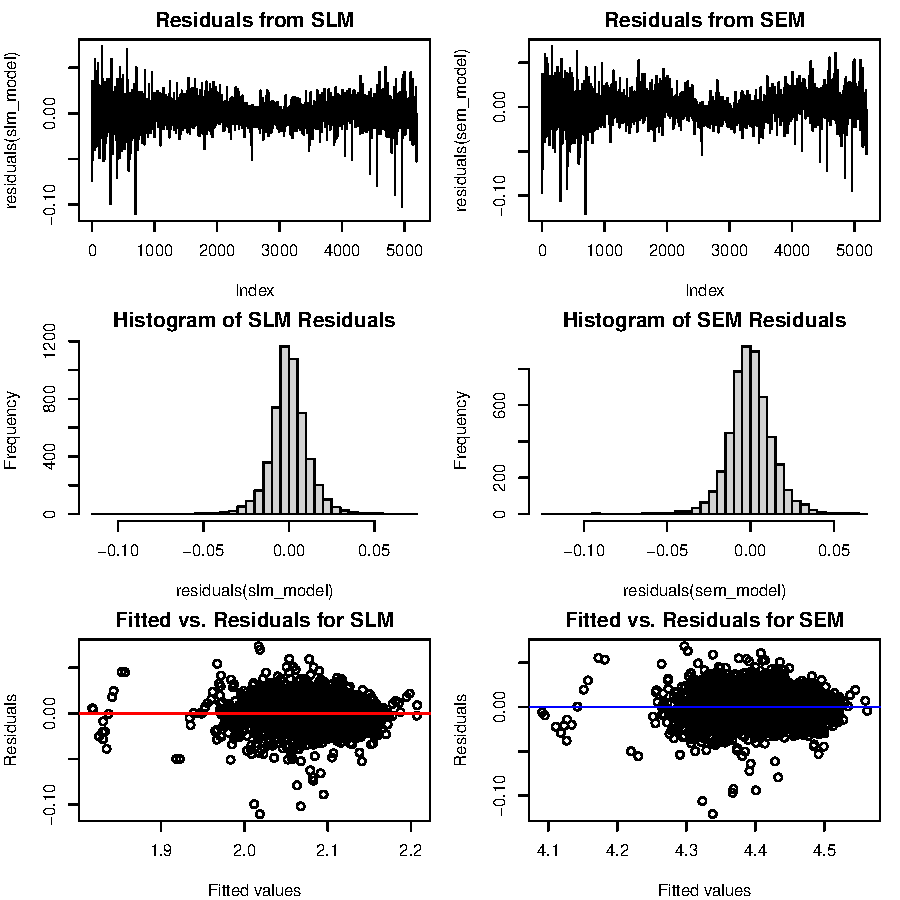
\includegraphics{S_E_Ampah_QRE-plot-diagnostics}
\end{subfigure}
\end{figure}
\end{frame}


\section{Conclusion}
\begin{frame}{Summary of Findings and Policy Implications}
\frametitle{Conclusion}

% Increase the space between lines
\setlength{\parskip}{1em}  

\textbf{Robustness of Findings:}
\begin{itemize}
  \setlength\itemsep{1em}  % Increase space between items
  \item \textbf{Consistent Variables:} HEEQ, HI, and UR consistently show significant effects across all models.
  \item \textbf{Spatial Effects:} Both SLM and SEM highlight significant spatial dependencies, underscoring the importance of incorporating spatial econometric techniques.
  \item \textbf{Household Income (HI):} Emerges as a critical factor, with both direct and spatial spillover effects significantly influencing employment rates.
\end{itemize}

\end{frame}


\begin{frame}{Policy Implications}
\frametitle{Conclusion}

% Increase the space between lines
\setlength{\parskip}{1em}  

\textbf{Policy Implications:}
\begin{itemize}
  \setlength\itemsep{1em}
  \item \textbf{Enhancing Education:} Addressing the negative impact of higher education enrollment on employment may involve aligning educational outcomes with market needs.
  \item \textbf{Supporting Knowledge-Intensive Industries:} Encouraging growth in these sectors can positively influence employment.
  \item \textbf{Boosting Household Income:} Policies aimed at increasing household income can have substantial direct and spillover benefits for regional employment.
  \item \textbf{Addressing Unemployment:} Targeted interventions are needed to mitigate structural unemployment and its regional impacts.
\end{itemize}

\end{frame}


% Bibliography
%%---------------------------------
\section{Bibliography}
\begin{frame}{References}
\small
\printbibliography
\end{frame}


\end{document}

